\documentclass[12pt]{article}

% ----------- PACKAGES -----------
\usepackage[utf8]{inputenc}
\usepackage{graphicx}
\usepackage{amsmath}
\usepackage{amssymb}
\usepackage{float}
\usepackage{hyperref}
\usepackage{caption}
\usepackage{booktabs}
\usepackage{tikz}
\usepackage{enumitem}
\usepackage{titlesec}
\usepackage{svg}
% \usepackage{cite}
\usepackage[margin=1in]{geometry}
\usepackage{siunitx}
\usepackage{pgfplots}
\usepackage{pdfpages}
\usepackage{subcaption}

% ----------- FORMATTING -----------
\setlength{\parskip}{0.5em}
\setlength{\parindent}{0pt}
\captionsetup{font=small}
\renewcommand{\figurename}{Figure}
\renewcommand{\tablename}{Table}


% ----------- TITLE -----------
\title{ECSE-4320 Project 1 \\ \large SIMD Advantage Profiling}
\author{Timon Cappella-Pimor}
\date{\today}

% ==================================
\begin{document}
% \pagenumbering{gobble}
\maketitle
\newpage
\section*{Methodology}

The benchmark suite is written in C, with one harness program that handles random data generation, dispatches and times the kernels, then outputs data over stdout in CSV format. Each kernel (SAXPY, Elementwise multiply, and 1D three-point stencil) has three versions: 1-stride, n-stride, and gather. Splitting the functions based on stride allows the compiler to better optimize for memory access patterns. The harness selects which one to run at run-time depending on command-line flags.

Each test begins by running the selected kernel 3 times over the full test data to warm up the system (cache, SIMD units, branch predictor, etc.), begins timing (using \\ \texttt{clock\_gettime(CLOCK\_MONOTONIC)} for nano-second precision), runs the kernel 10 more times, stops timing, then reports the time per kernel and computed values (throughput, memory bandwidth, etc.). This entire process is repeated 10 times yielding 10 rows in the CSV table, and the first one is discarded for data analysis and plotting. The exact series of benchmarks can be found in \texttt{run\_tests.sh}.

Test data are all regular floating point values (no sub-normals) between -1 and 1 pre-generated using a seeded PRNG, and cached in a file. If the file contains sufficiently many values for the requested working set size, then it will be read and used directly as the inputs. Otherwise, the harness will expand the cache file to match the working set size. All tests ran with the same seed using the same data cache. Note that single- and double-precision tests need separate data caches.

Assume all tests involve cache-line-aligned, single-precision elements with a unit-stride access pattern unless stated otherwise.

All three harnesses were compiled locally on the benchmark machine with GCC 16.2.1 under the c23 standard. Vectorization is set at compile time using these flags:
\begin{itemize}
    \item scalar: \texttt{-O3 -fno-tree-vectorize}

    \item autovec\_default (SSE2): \texttt{-O3}

    \item autovec\_widest (AVX-512): \texttt{-O3 -march=native}
\end{itemize}


Linux Kernel Version: 7.2.11-zen1-1-zen \\
CPU: AMD Ryzen 7 9700X (Core 0) \\
Caches: L1d 48KB, L2 1024KB, L3 32MB \\
Max Clock Speed: 5.58 GHz \\
Governor: Performance

\newpage
\section*{Vectorization Verification}




\newpage
\section*{Locality and Memory-bound Analysis}
\begin{figure}[H]
    \centering

    % Row 1
    \begin{subfigure}[b]{0.48\textwidth}
        \centering
        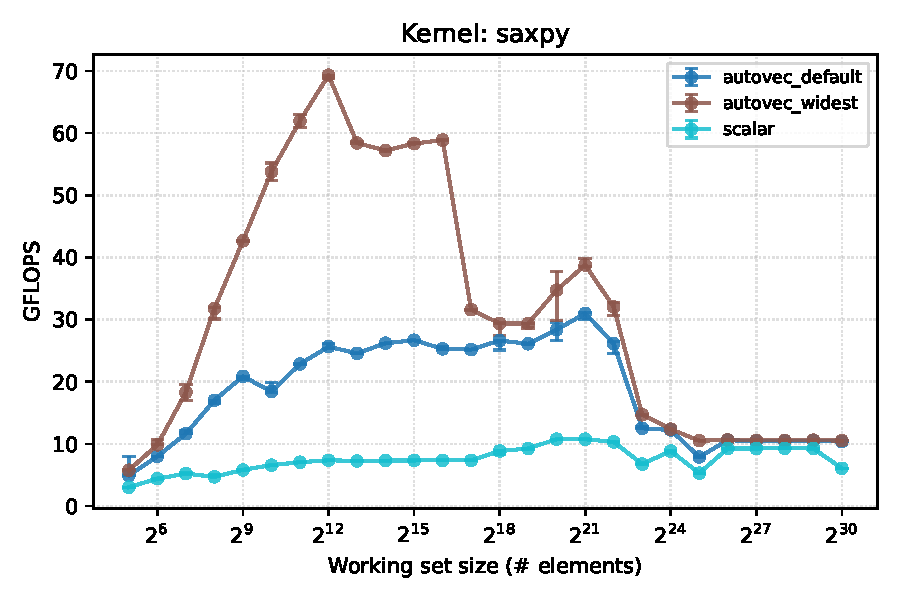
\includegraphics[width=\linewidth]{../plots/flops_saxpy.pdf}
        \caption{SAXPY Throughput}
        \label{fig:flops_saxpy}
    \end{subfigure}
    \hfill
    \begin{subfigure}[b]{0.48\textwidth}
        \centering
        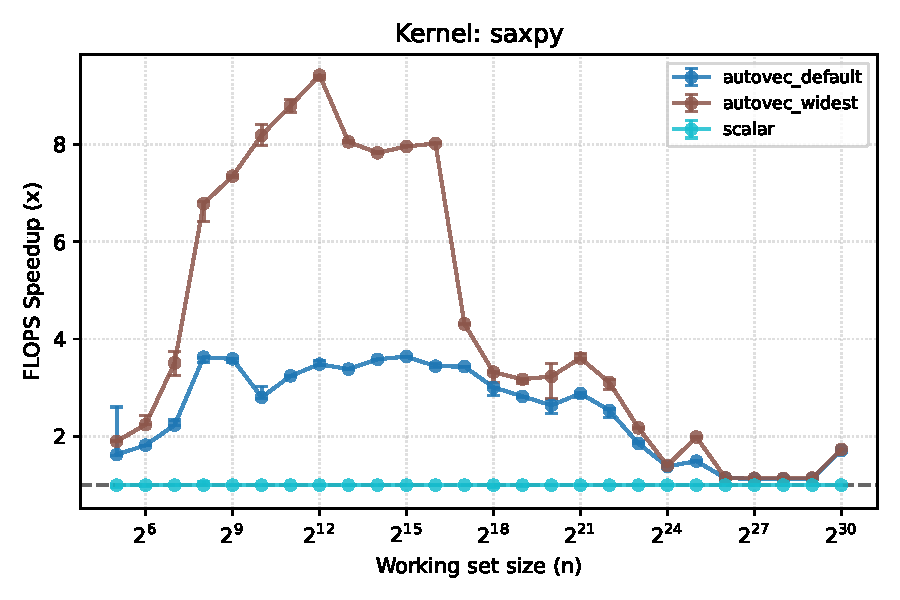
\includegraphics[width=\linewidth]{../plots/speedup_saxpy.pdf}
        \caption{SAXPY Speedup}
        \label{fig:speedup_saxpy}
    \end{subfigure}


    \vspace{0.3cm}

    % Row 2
    \begin{subfigure}[b]{0.48\textwidth}
        \centering
        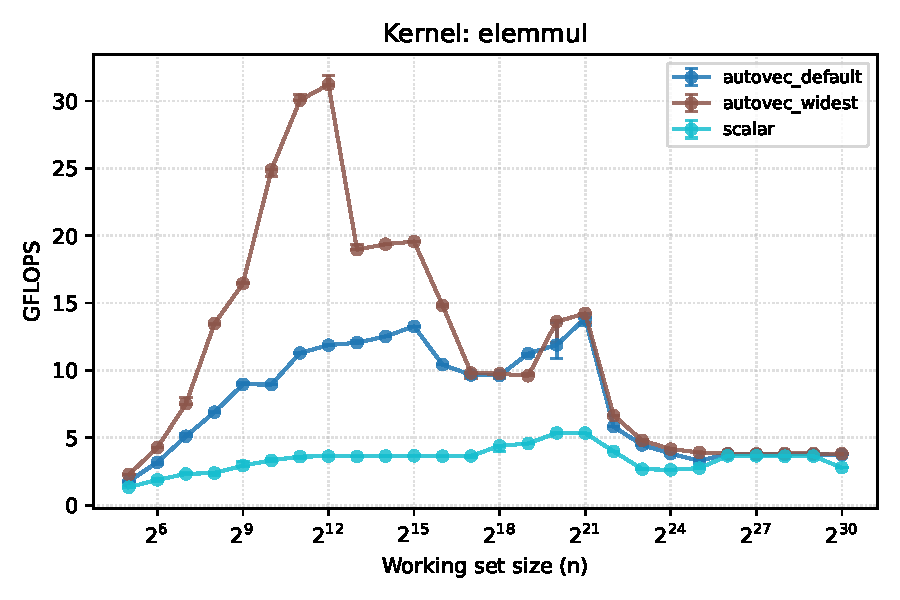
\includegraphics[width=\linewidth]{../plots/flops_elemmul.pdf}
        \caption{Elem-mul Throughput}
        \label{fig:flops_elemmul}
    \end{subfigure}
    \hfill
    \begin{subfigure}[b]{0.48\textwidth}
        \centering
        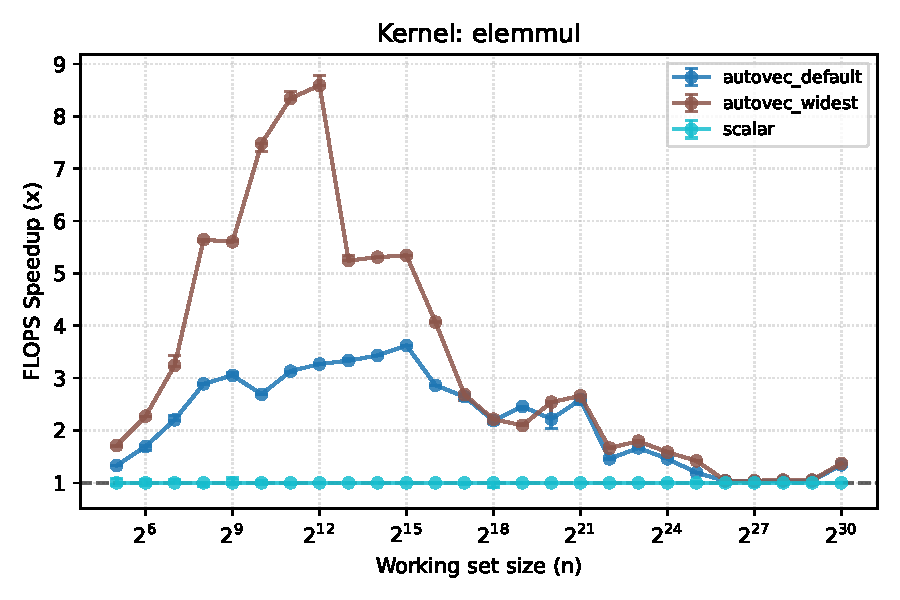
\includegraphics[width=\linewidth]{../plots/speedup_elemmul.pdf}
        \caption{Elem-mul Speedup}
        \label{fig:speedup_elemmul}
    \end{subfigure}

    \vspace{0.3cm}

    % Row 3
    \begin{subfigure}[b]{0.48\textwidth}
        \centering
        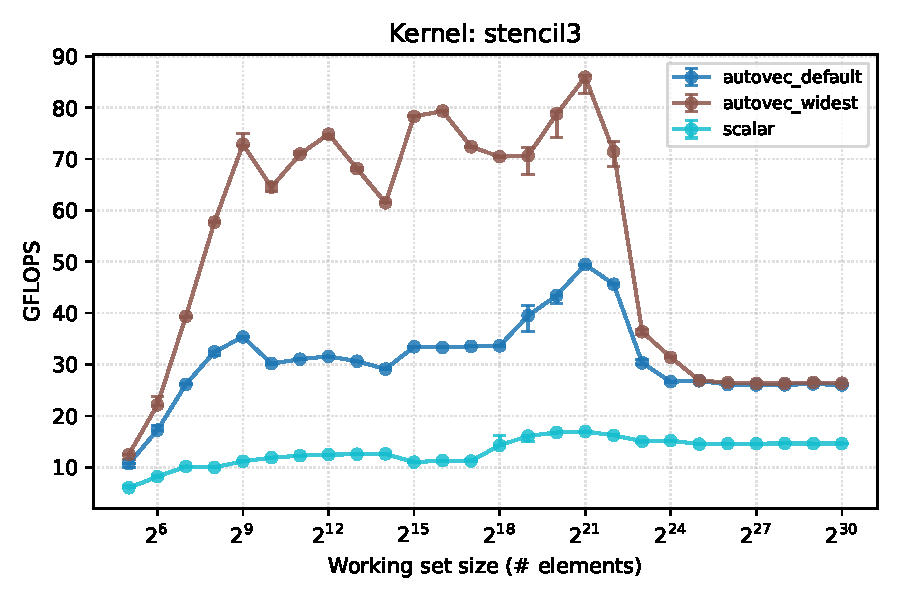
\includegraphics[width=\linewidth]{../plots/flops_stencil3.pdf}
        \caption{Stencil3 Throughput}
        \label{fig:flops_stencil}
    \end{subfigure}
    \hfill
    \begin{subfigure}[b]{0.48\textwidth}
        \centering
        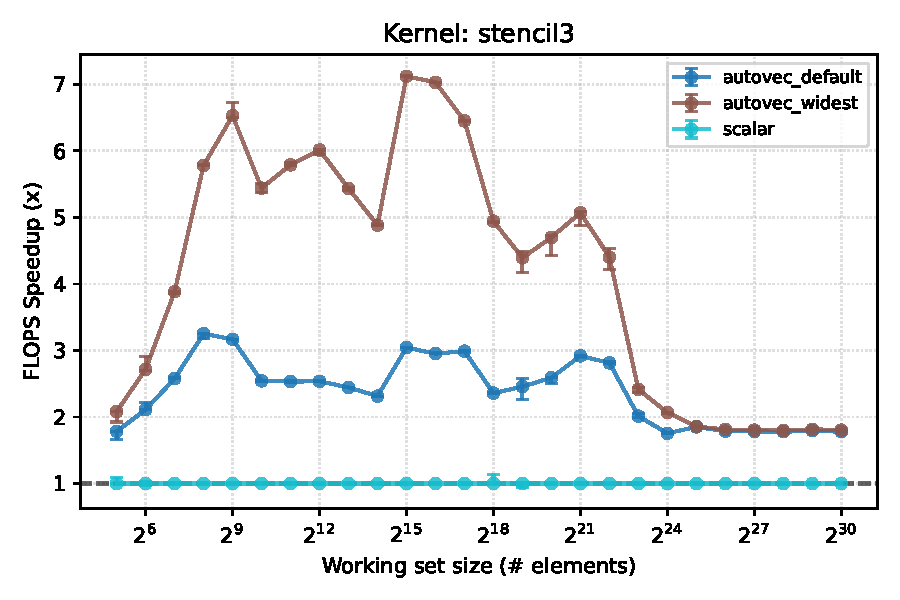
\includegraphics[width=\linewidth]{../plots/speedup_stencil3.pdf}
        \caption{Stencil3 Speedup}
        \label{fig:speedup_stencil}
    \end{subfigure}

    \caption{Performance results versus working size for SAXPY, element-wise
    multiplication, and Stencil3. The left column shows raw throughput, while
    the right column shows the speedup as a multiple of scalar performance.}
    \label{fig:performance_results}
\end{figure}

We will first examine SAXPY and Elem-mul, as their structure is similar (two reads, followed by one write). Under the assumption that memory bandwidth will be their biggest bottleneck, we should expect to see sharp drops in performance as $n$ grows larger than a cache's size. SAXPY uses 8 bytes of memory for each $n$, wheras Elem-mul uses 12 bytes. Based on the cache sizes and $n$'s growth in powers of 2, we should expect to see transitions at $n = 2^{13}$ (L1 to L2), $2^{17}$ (L2 to L3), and $2^{22}$ (L3 to DRAM).

In fact, this is exactly what we see. Throughput grows to peaks of 70 and 31 GFLOPS (9x speedup) at $2^{12}$ elements for SAXPY and Elem-mul respectively. In this regime, runtime is likely dominated by initialization overhead and pipeline latency for the vector processor. Each additional element contributes minimally to runtime, as reading from and writing to L1 cache is fast enough (sub-nanosecond) to keep the vector processor busy.

At $2^{13}$ elements, performance drops down to 58 and 19 GFLOPS respectively. Around one third of the data no longer fits in L1 cache, so the CPU must read and write back some data to L2, which is farther from the core and thus has higher latency than L1. Because Elem-mul accesses 12 bytes per element while SAXPY only accesses 8, Elem-mul is more significantly affected by the increased memory latency, so its throughput drops by a greater percentage than that of SAXPY's drop. Within this regime, throughput is limited by memory bandwidth and stays mostly constant.



\section*{Alignment, Tail, Stride/Gather Studies}

\begin{figure}[H]
    \makebox[\textwidth][c]{%
        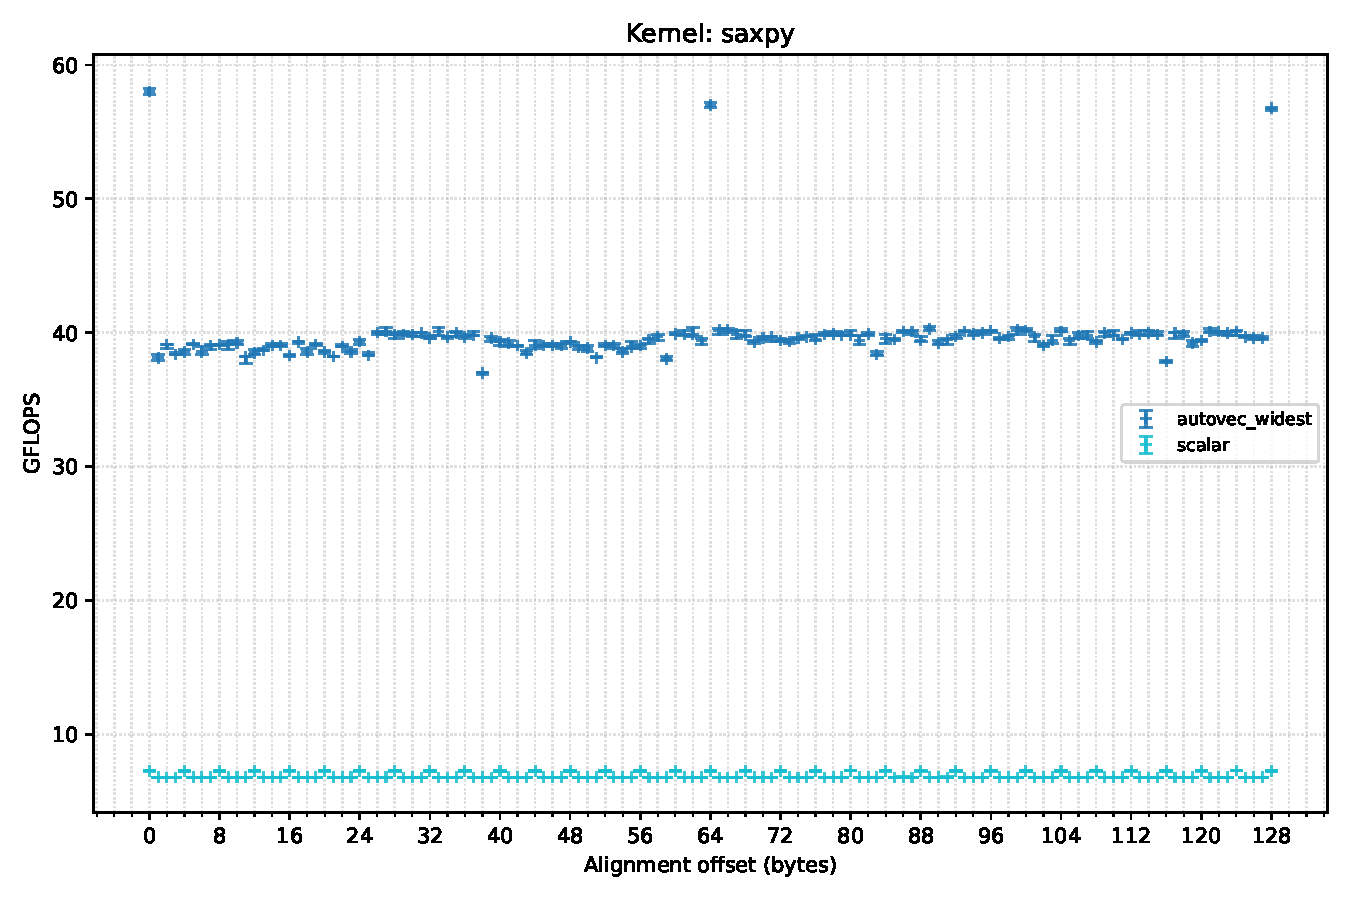
\includegraphics[width=\linewidth]{../plots/alignment_saxpy.pdf}%
    }
    \caption{SAXPY Throughput vs. Alignment}
    \label{fig:alignment}
\end{figure}

\begin{figure}[H]
    \makebox[\textwidth][c]{%
        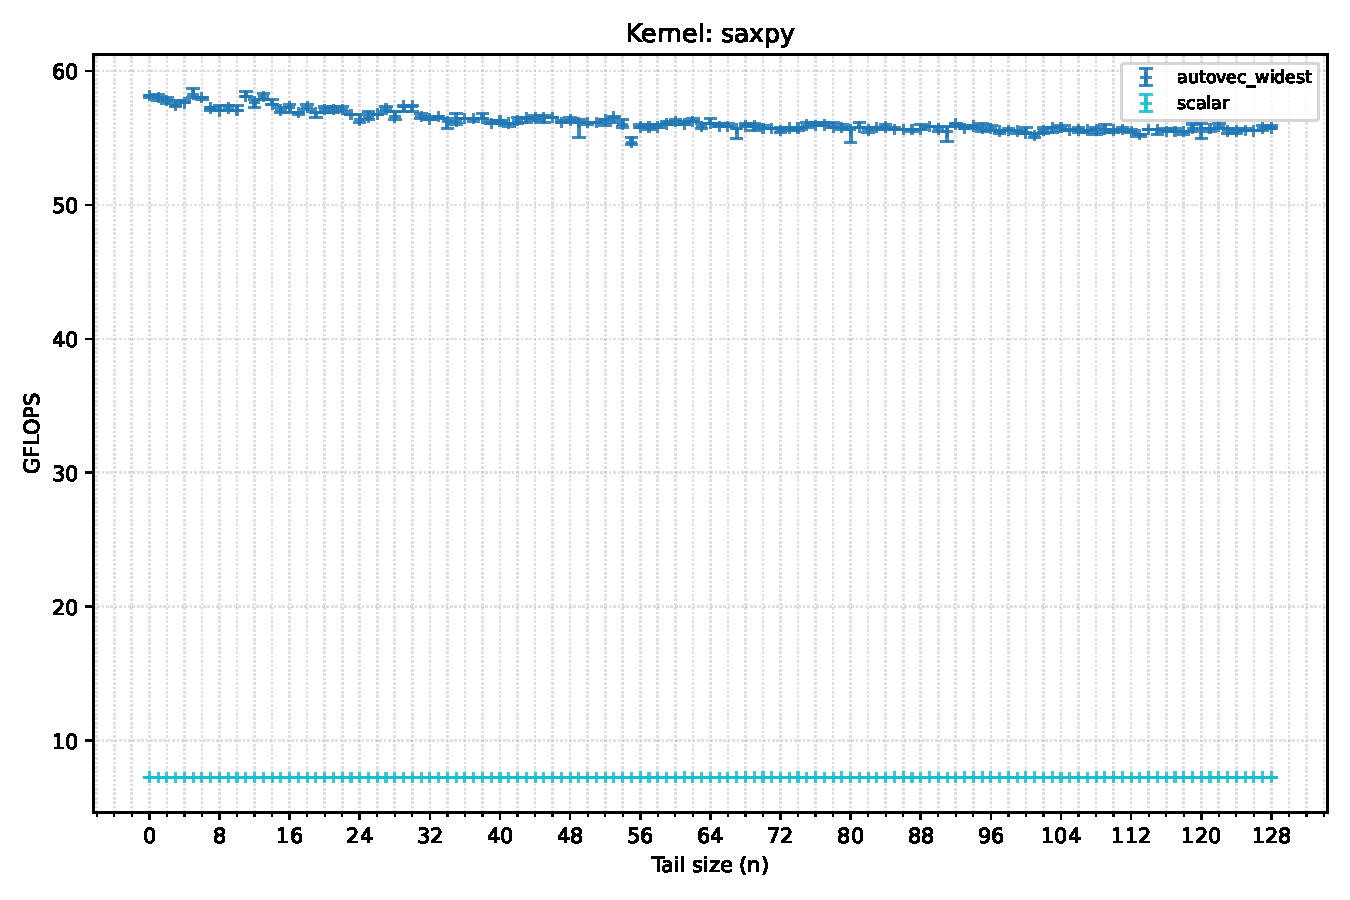
\includegraphics[width=\linewidth]{../plots/tail_saxpy.pdf}%
    }
    \caption{SAXPY Throughput vs. Tail Size}
    \label{fig:tail}
\end{figure}

\begin{figure}[H]
    \makebox[\textwidth][c]{%
        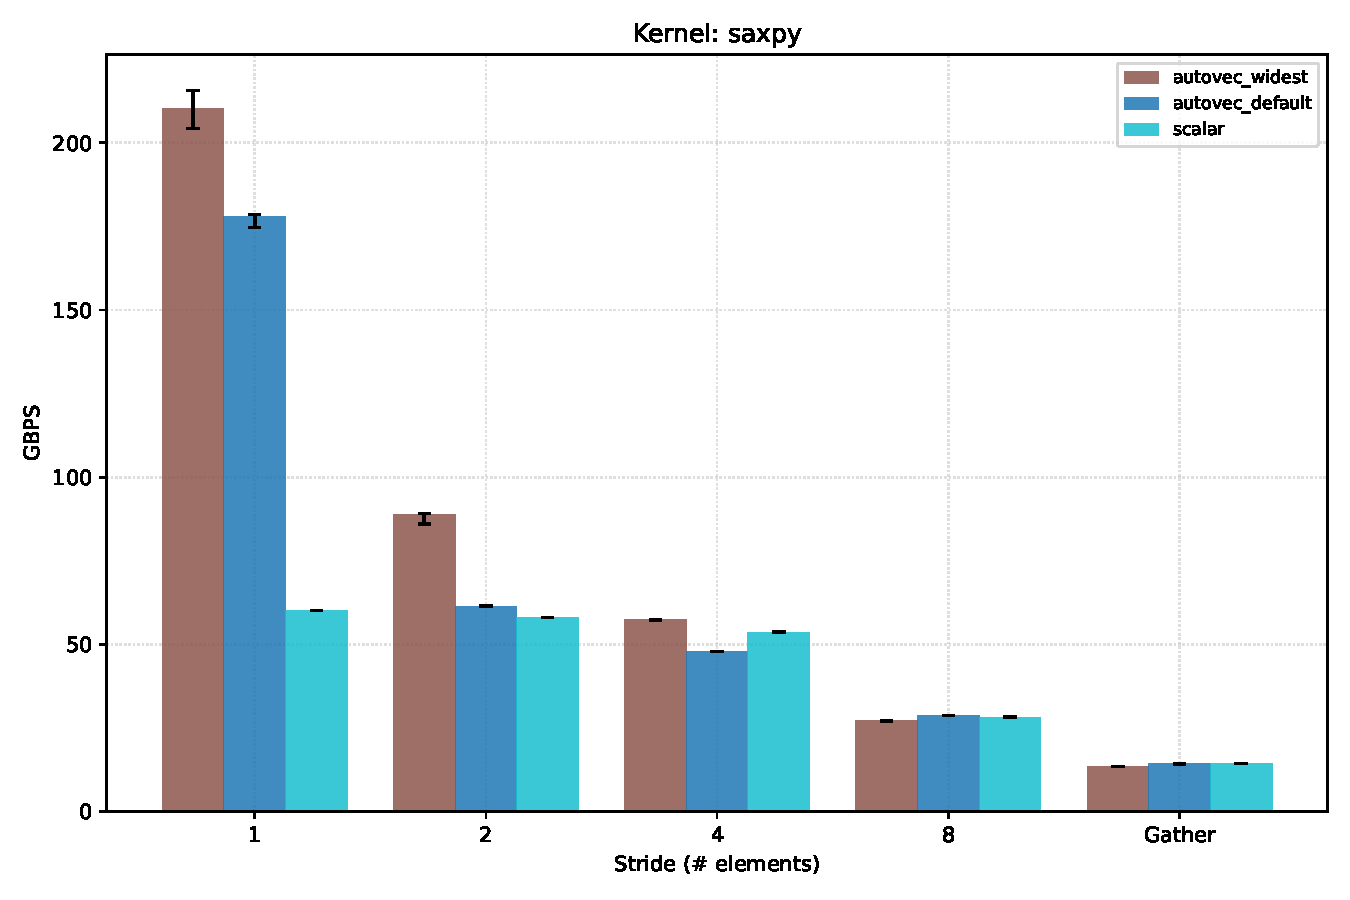
\includegraphics[width=\linewidth]{../plots/stride_saxpy.pdf}%
    }
    \caption{SAXPY Bandwidth vs. Stride}
    \label{fig:stride}
\end{figure}

\section*{Data-type Comparison}

\begin{figure}[H]
    \makebox[\textwidth][c]{%
        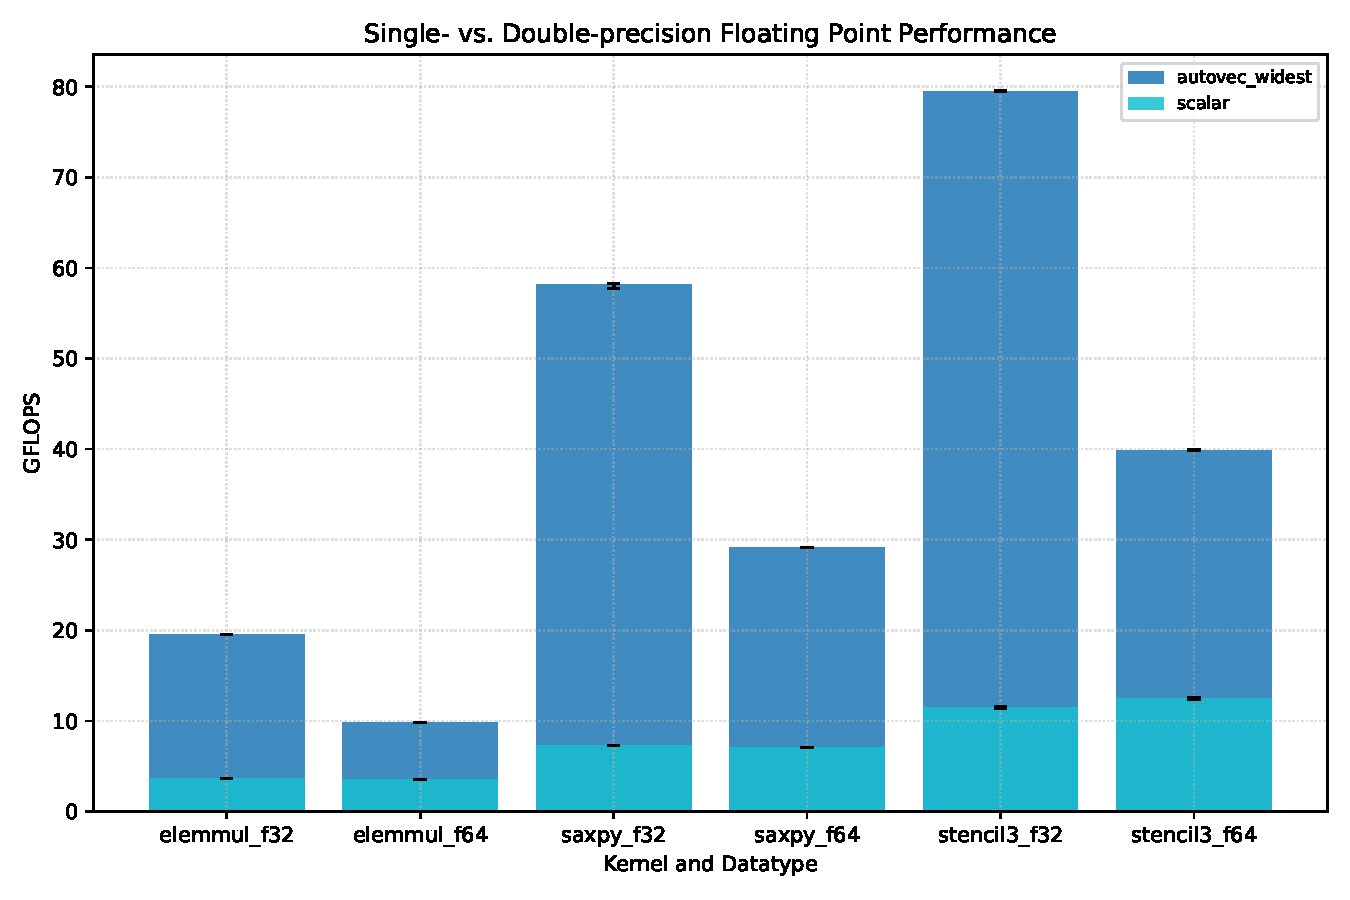
\includegraphics[width=\linewidth]{../plots/datatype.pdf}%
    }
    \caption{}
    \label{fig:datatype}
\end{figure}

\section*{Roofline and Quantitative Analysis}
\section*{AI-use Transparency and Failure Case}

Claude Sonnet 5.5 was used to write an initial pass of the benchmark code, as well as a few short snippets of Python code for some of the plots.

% ---- References ----
% \newpage
% \bibliographystyle{IEEEtran}
% \bibliography{references}

\end{document}
